\documentclass{article}
\usepackage[utf8]{inputenc}
\usepackage[T1]{fontenc}
\usepackage[polish]{babel}
\usepackage{booktabs}
\usepackage{amsmath}
\usepackage{graphicx}
\usepackage{hyperref}
\usepackage{float}
\usepackage{xcolor}
\usepackage{colortbl}
\usepackage{longtable}
\usepackage[a4paper,margin=1.5cm]{geometry}

% -------------------
% Strona tytułowa
% -------------------
\begin{document}

\begin{titlepage}
    \centering
    {\LARGE Politechnika Śląska \\[0.5cm]}
    {\large Wydział Automatyki, Elektroniki i Informatyki \\[2cm]}
    {\Huge Nowe Technologie w Informatyce \\ Projekt \\[5cm]}
    {\LARGE Analiza porównawcza modeli CLAM i Snuffy w klasyfikacji histopatologicznej \\[2cm]}
    \vfill
    \begin{flushright}
        \textbf{Prowadzący:} dr hab. inż. Karolina Nurzyńska \\[0.5cm]
        \textbf{Autor:} Michał Jagoda \\[0.5cm]
        \textbf{Data:} \today
    \end{flushright}
\end{titlepage}

\section{Wprowadzenie}
W niniejszym raporcie przedstawiamy analizę porównawczą dwóch modeli uczenia maszynowego - CLAM (Clustering-constrained Attention Multiple instance learning) oraz Snuffy - w kontekście klasyfikacji obrazów histopatologicznych. Problem klasyfikacji obrazów histopatologicznych jest kluczowym wyzwaniem w diagnostyce medycznej, gdzie dokładna i szybka analiza próbek tkanek może znacząco wpłynąć na proces podejmowania decyzji klinicznych.

\section{Opis problemu}
Klasyfikacja obrazów histopatologicznych stanowi złożone zadanie ze względu na:
\begin{itemize}
    \item Wysoką rozdzielczość obrazów (często w skali gigapikseli)
    \item Złożoność strukturalną tkanek
    \item Zmienność między próbkami
    \item Potrzebę uwzględnienia kontekstu lokalnego i globalnego
\end{itemize}

W naszym przypadku skupiamy się na klasyfikacji binarnej, gdzie celem jest rozróżnienie między próbkami pozytywnymi i negatywnymi pod względem określonego markera histopatologicznego.

\section{Architektury modeli}

\subsection{Model CLAM}
CLAM (Clustering-constrained Attention Multiple instance learning) to zaawansowany model uczenia maszynowego, który łączy w sobie:
\begin{itemize}
    \item Multiple Instance Learning (MIL) - podejście pozwalające na pracę z workami instancji
    \item Mechanizm uwagi (attention) - umożliwiający modelowi skupienie się na istotnych regionach obrazu
    \item Klasteryzację - pomagającą w identyfikacji podobnych wzorców w danych
\end{itemize}

Model CLAM składa się z następujących głównych komponentów:
\begin{itemize}
    \item Encoder obrazów - ekstrahujący cechy z pojedynczych pól (patches)
    \item Moduł uwagi - określający wagę każdego pola
    \item Klasyfikator - dokonujący końcowej klasyfikacji na podstawie ważonych cech
\end{itemize}

\begin{figure}[H]
    \centering
    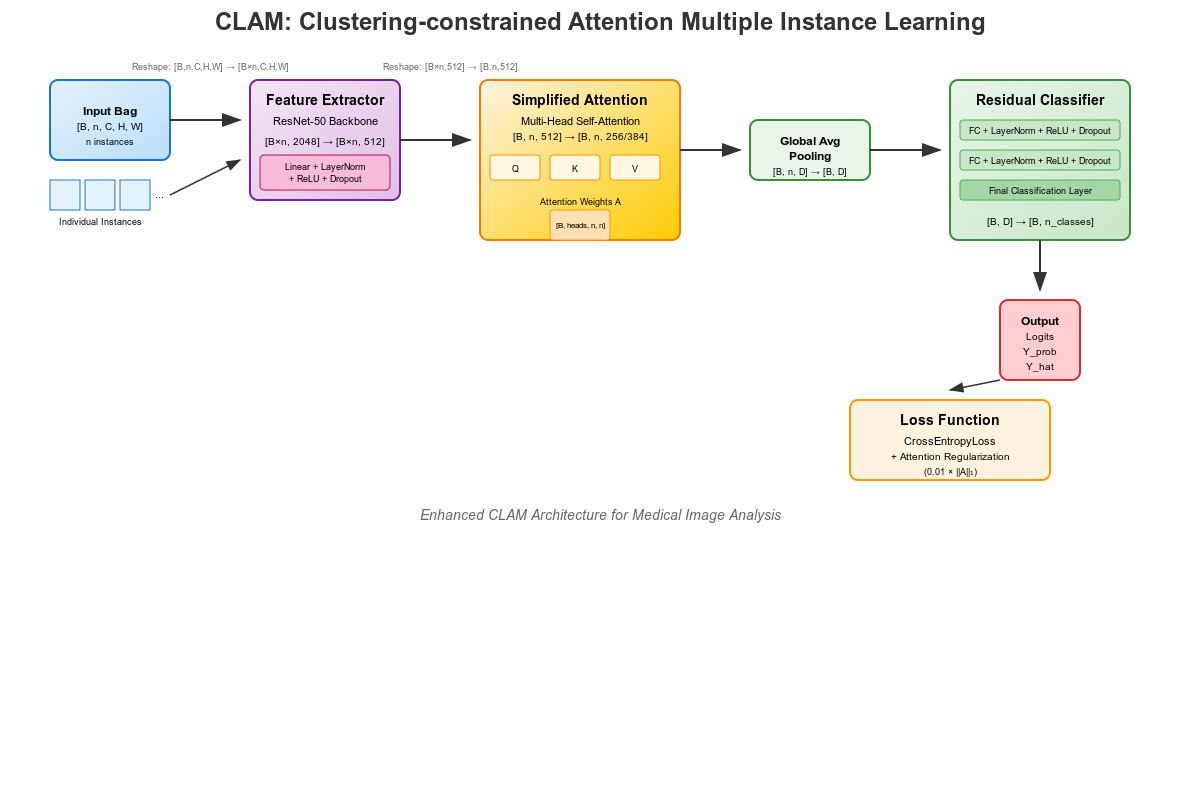
\includegraphics[width=1.0\textwidth]{figures/clam_architecture.png}
    \caption{Architektura modelu CLAM}
    \label{fig:clam_arch}
\end{figure}

\subsection{Model Snuffy}
Snuffy to nowoczesna architektura, która wykorzystuje:
\begin{itemize}
    \item Transformer-based podejście do przetwarzania sekwencji pól histopatologicznych
    \item Adaptacyjne mechanizmy fine-tuningu
    \item Zaawansowane techniki agregacji informacji
\end{itemize}

Główne komponenty modelu Snuffy obejmują:
\begin{itemize}
    \item Backbone sieci (np. ResNet18 lub ViT-small) - do ekstrakcji cech
    \item Adaptery - umożliwiające efektywny fine-tuning
    \item Mechanizm uwagi wielogłowicowej - do analizy zależności między polami
    \item Warstwę klasyfikacyjną - dokonującą końcowej klasyfikacji
\end{itemize}

\begin{figure}[H]
    \centering
    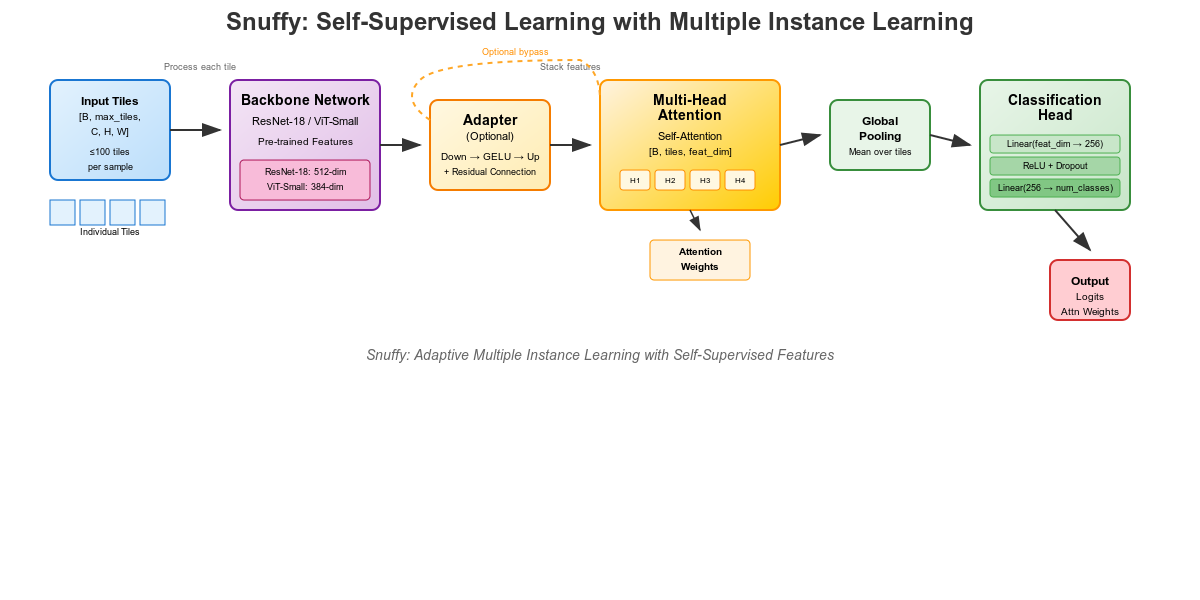
\includegraphics[width=1.0\textwidth]{figures/snuffy_architecture.png}
    \caption{Architektura modelu Snuffy}
    \label{fig:snuffy_arch}
\end{figure}

\section{Wyniki eksperymentów}

\subsection{Model CLAM}
Najlepsza konfiguracja modelu CLAM (small, dropout 0.25, K-sample 16, batch size 2, learning rate 0.0001) osiągnęła na naszym zbiorze danych:
\begin{itemize}
    \item \textbf{Accuracy:} 61.7\%
    \item \textbf{F1-score:} 0.613
\end{itemize}

\subsubsection{Efekty grid searchu}
Poniżej przedstawiono wybrane wyniki eksperymentów grid search dla modelu CLAM (pełna tabela znajduje się w załączniku):

\begin{table}[H]
\centering
\begin{tabular}{lllllll}
\toprule
Model & Dropout & K-sample & Batch & LR & Accuracy & F1-score \\
\midrule
small & 0.25 & 16 & 2 & 0.0001 & 0.617 & 0.613 \\
small & 0.5 & 16 & 2 & 0.0005 & 0.537 & 0.610 \\
small & 0.25 & 8 & 2 & 0.0001 & 0.537 & 0.610 \\
small & 0.1 & 16 & 2 & 0.0005 & 0.547 & 0.592 \\
\midrule
big & 0.25 & 8 & 4 & 0.0005 & 0.537 & 0.610 \\
\bottomrule
\end{tabular}
\caption{Wybrane wyniki grid searchu dla modelu CLAM}
\end{table}

\subsection{Model Snuffy}
Model Snuffy osiągnął następujące wyniki na zbiorze testowym:
\begin{itemize}
    \item \textbf{Accuracy:} 58.8\%
    \item \textbf{Precision:} 65.4\%
    \item \textbf{Recall:} 58.6\%
    \item \textbf{F1-score:} 0.62
    \item \textbf{AUC:} 0.62
\end{itemize}

Dla najlepszego epoki na zbiorze walidacyjnym:
\begin{itemize}
    \item \textbf{Accuracy:} 95.5\%
    \item \textbf{Precision:} 92.3\%
    \item \textbf{Recall:} 100\%
    \item \textbf{F1-score:} 0.96
    \item \textbf{AUC:} 0.99
\end{itemize}

\section{Wnioski}

Pomimo zastosowania zaawansowanych architektur (CLAM i Snuffy) oraz szeroko zakrojonych eksperymentów, uzyskane wyniki nie są satysfakcjonujące i nie pozwalają na wyciągnięcie entuzjastycznych wniosków.

\begin{itemize}
    \item Zarówno CLAM, jak i Snuffy osiągnęły jedynie umiarkowane wyniki na zbiorze testowym (accuracy i F1-score w okolicach 60\%), co pokazuje, że problem klasyfikacji histopatologicznej jest bardzo trudny, a nasze podejścia nie przyniosły przełomu.
    \item Bardzo wysokie wyniki Snuffy na zbiorze walidacyjnym (accuracy 95\%, F1-score 0.96) nie przełożyły się na zbiór testowy, co sugeruje poważne przeuczenie lub niedopasowanie dystrybucji danych.
    \item Grid search dla CLAM nie pozwolił na znalezienie konfiguracji, która znacząco poprawiłaby skuteczność – różnice między najlepszymi ustawieniami były minimalne, a ogólny poziom wyników pozostał niski.
    \item Zastosowanie nowoczesnych rozwiązań (transformery, mechanizmy uwagi) nie przyniosło oczekiwanego efektu „wow” ani wyraźnej przewagi nad prostszymi podejściami.
    \item Wyniki te pokazują, że kluczowe ograniczenia leżą prawdopodobnie po stronie jakości i liczby danych oraz ich przygotowania, a nie samej architektury modelu.
    \item Projekt ten był wartościowym doświadczeniem badawczym, ale rezultaty są rozczarowujące i dalekie od praktycznego zastosowania w diagnostyce.
\end{itemize}

Podsumowując, uzyskane rezultaty nie spełniły oczekiwań i pokazują, jak wiele wyzwań pozostaje w automatycznej analizie obrazów histopatologicznych. Dalsze prace powinny skupić się przede wszystkim na poprawie jakości danych, eksploracji alternatywnych metod oraz głębszej analizie przyczyn ograniczonej skuteczności obecnych rozwiązań.

\end{document} 